% =====================================================================
% paper.tex
% From Natural Language to Verifiable Reasoning:
% A Semantic Reduction Framework for Reliable AI Mathematics
%
% 编译方式（任选其一）：
%   pdflatex paper.tex && bibtex paper && pdflatex paper.tex && pdflatex paper.tex
%   xelatex 同上
%   tectonic paper.tex   （一步完成，含 BibTeX）
%
% 本文件不依赖任何本地图片；图 1 为 TikZ 绘制。
% =====================================================================
\documentclass[11pt,a4paper]{article}

\usepackage[margin=2.6cm]{geometry}
\usepackage{amsmath,amssymb,amsthm}
\usepackage{booktabs}
\usepackage{multirow}
\usepackage[numbers,sort&compress]{natbib}
\usepackage{tikz}
\usetikzlibrary{arrows.meta,positioning}
\usepackage[colorlinks=true,linkcolor=blue!60!black,citecolor=blue!60!black,urlcolor=blue!60!black]{hyperref}

\newtheorem{observation}{Observation}
\newtheorem{definition}{Definition}

\newcommand{\ir}{\mathsf{IR}}
\newcommand{\nl}{\mathsf{NL}}

\title{\textbf{From Natural Language to Verifiable Reasoning:\\
A Semantic Reduction Framework for Reliable AI Mathematics}}
\author{C2 Project}
\date{October 2026}

\begin{document}
\maketitle

% =====================================================================
\begin{abstract}
Large language models (LLMs) now produce fluent, confident-looking mathematical reasoning, yet a growing body of evidence shows that such output can be locally plausible and globally wrong: intermediate steps may be invalid even when final answers are correct, and final answers may be correct while the reasoning is not. Existing responses fall into three families---search over generated candidates, independent verification, and fully formal proving. We argue that this view, organized around \emph{where} reliability is enforced, obscures the more decisive question of \emph{what} is actually being verified. We propose a three-layer model of AI mathematical reasoning (generation, semantic reduction, verification) and identify the \emph{semantic reduction layer}---the mapping from natural language to verifiable structured objects---as the central bottleneck of current systems. We contribute (i) a failure-mode taxonomy of this layer (ambiguity, type incompleteness, non-invertibility, vacuous formalization, and format drift), grounded in published case studies; (ii) a cross-paper comparative analysis of four verification architectures along the dimensions of what is verified, the strength of the guarantee, and observed failure rates, using only previously published numbers; and (iii) a practical 12-item reliability checklist (SRC-12) for assessing AI-generated mathematical conclusions. We close with the boundary conditions of our claims and a discussion of what evidence would falsify the framework.
\end{abstract}

% =====================================================================
\section{Introduction}\label{sec:intro}

LLMs such as GPT-4 and Minerva have demonstrated striking performance on mathematical benchmarks: Minerva surpasses 50\% accuracy on the MATH competition dataset \citep{hendrycks2021math,lewkowycz2022minerva}, and CoT-style prompting substantially lifts multi-step reasoning accuracy across model scales \citep{wei2022cot}. At the same time, careful audits reveal systematic weaknesses. \citet{frieder2023chatgpt} find that ChatGPT's self-reported confidence correlates poorly with actual correctness on university-level mathematics, and \citet{uesato2022feedback} show that among solutions whose \emph{final answers} are correct, a substantial fraction contain invalid reasoning steps when humans read them. In other words, the quantity most benchmarks optimize---final-answer accuracy---is a weak proxy for the thing users actually need: \emph{trustworthy reasoning}.

The community's response can be summarized as a reliability triad: (1)~\emph{search}, e.g., best-of-$N$ sampling with majority voting \citep{cobbe2021gsm8k,lightman2024verify}; (2)~\emph{verification}, e.g., learned verifiers \citep{cobbe2021gsm8k}, process reward models \citep{uesato2022feedback,lightman2024verify}, and autoformalization followed by automated theorem provers \citep{zhou2024dtv}; and (3)~\emph{formal proving}, in which the reasoning itself is carried out inside a proof assistant such as Lean \citep{demoura2021lean4}, culminating in systems like AlphaGeometry \citep{trinh2024alphageometry} and AlphaProof \citep{hubert2025alphaproof} that reach medal-level performance on olympiad problems.

These three directions are usually presented as alternative mechanisms. We argue that they are better understood as different placements of the \emph{same} missing component: a stable mapping between informal natural-language mathematics and formal, machine-checkable objects. Pure search operates entirely downstream of this mapping; learned verifiers approximate it with neural networks; formal systems eliminate it only by moving the whole workflow into a formal language that few practitioners use. The reliability question therefore concentrates on this mapping, which we call the \emph{semantic reduction layer}.

\paragraph{Contributions.} This paper makes three modest but, to our knowledge, non-redundant contributions:
\begin{enumerate}
  \item \textbf{A three-layer model} (generation, semantic reduction, verification) that reorganizes the reliability triad around the object being verified, with an explicit failure-mode taxonomy of the reduction layer (\S\ref{sec:model}--\S\ref{sec:bottleneck}).
  \item \textbf{A cross-paper comparative analysis} of four verification architectures---outcome verifiers, process reward models, autoformalization-then-ATP, and formal RL provers---using only numbers published in the original papers, making explicit which claims survive the change of benchmark and which do not (\S\ref{sec:analysis}).
  \item \textbf{SRC-12}, a 12-item reliability checklist that operationalizes the three-layer model for practitioners who must decide \emph{today} whether to trust an AI-generated mathematical conclusion (\S\ref{sec:framework}).
\end{enumerate}

We state our scope honestly: this is a position-and-analysis paper, not a systems paper. We run no new models. All quantitative evidence is quoted from the cited primary literature; where numbers are not comparable across papers, we say so (\S\ref{sec:limits}).

% =====================================================================
\section{A Three-Layer Model of AI Mathematical Reasoning}\label{sec:model}

\begin{definition}[Semantic reduction]
Let $\nl$ denote the space of natural-language mathematical statements and $\ir$ a space of typed, machine-checkable objects (logical formulas, programs, or proof obligations). A \emph{semantic reduction} is a partial function
\begin{equation}
\rho : \nl \rightharpoonup \ir ,
\label{eq:rho}
\end{equation}
defined only on statements whose informal meaning admits a faithful formal counterpart. Reliability of a system $S$ that answers natural-language mathematical questions depends on $\rho$ being \emph{defined} (the reduction succeeds) and \emph{faithful} (the formal object preserves the intended meaning).
\end{definition}

The partiality in~\eqref{eq:rho} is where much of the practical difficulty lives. The three-layer model is then:

\begin{enumerate}
  \item \textbf{Generation layer.} An LLM produces natural-language reasoning (typically chain-of-thought). Outputs are probabilistic, untyped, and informal; correctness is not guaranteed at any granularity \citep{wei2022cot,lewkowycz2022minerva}.
  \item \textbf{Semantic reduction layer.} Reasoning is mapped to structured objects: executable programs \citep{gao2023pal,chen2023pot}, tool calls \citep{schick2023toolformer}, formal statements \citep{zhou2024dtv}, or proof obligations in Lean/Isabelle \citep{jiang2023draft,yang2023leandojo}. Theoretical grounding comes from the Curry--Howard correspondence: a verifiable object corresponds to an explicit proof term, whereas natural language does not.
  \item \textbf{Verification layer.} The structured object is checked: consistency (internal), derivability (proof obligations discharged in a formal system), factual grounding (constraint satisfaction, or comparison with references), or constraint satisfaction (solvers). Tools range from SMT solvers to Lean 4 \citep{demoura2021lean4}.
\end{enumerate}

\begin{figure}[t]
\centering
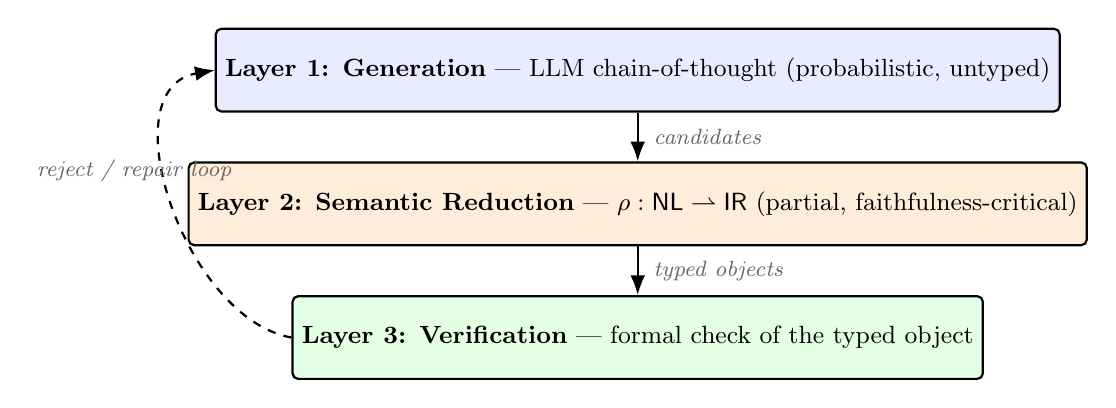
\begin{tikzpicture}[
  layer/.style={rectangle,rounded corners=2pt,draw,thick,minimum width=8.6cm,minimum height=1.05cm,align=center,font=\small},
  side/.style={font=\footnotesize\itshape,text=black!60,align=left},
  arr/.style={-{Latex[length=2.5mm]},thick},
  node distance=0.62cm and 1.1cm]
  \node[layer,fill=blue!8]   (gen)  {\textbf{Layer 1: Generation} --- LLM chain-of-thought (probabilistic, untyped)};
  \node[layer,fill=orange!14,below=of gen] (red) {\textbf{Layer 2: Semantic Reduction} --- $\rho:\nl\rightharpoonup\ir$ (partial, faithfulness-critical)};
  \node[layer,fill=green!10,below=of red]  (ver) {\textbf{Layer 3: Verification} --- formal check of the typed object};
  \draw[arr] (gen) -- node[right,side,xshift=2pt]{candidates} (red);
  \draw[arr] (red) -- node[right,side,xshift=2pt]{typed objects} (ver);
  \draw[arr,dashed] (ver.west) to[out=170,in=190] node[above,side,xshift=-14pt,yshift=4pt]{reject / repair loop} (gen.west);
\end{tikzpicture}
\caption{The three-layer reliability model. The dashed loop is the feedback path used by search-and-repair systems. Our central claim (\S\ref{sec:bottleneck}) is that observed failures concentrate at Layer 2: the reduction $\rho$ is either undefined (nothing to verify) or unfaithful (the wrong thing is verified).}
\label{fig:threelayer}
\end{figure}

% =====================================================================
\section{The Semantic Reduction Bottleneck: A Failure-Mode Taxonomy}\label{sec:bottleneck}

If Layer 3 is given a well-typed, faithful object, verification is essentially solved---formal proof checking is decidable and cheap. The difficult question is whether $\rho$ ever produces such an object. Drawing on published case studies and failure analyses, we classify Layer-2 failures into five modes:

\begin{description}
  \item[F1. Ambiguity.] Informal statements admit multiple formal readings; the LLM commits to one silently. \citet{frieder2023chatgpt} document cases where a problem statement is ``corrected'' by the model before solving, i.e., the model answers a different question than the one asked.
  \item[F2. Type incompleteness.] Natural language omits domain information that formal systems require. \citet{zhou2024dtv} report an Isabelle translation mistaking $(1::\mathrm{nat})^2$ for $1^2$ where the type annotation changes the result---an error invisible at the natural-language level.
  \item[F3. Non-invertibility.] Reduction loses information: two different informal solutions can map to the same $\ir$ object, or a formal object can correspond to unintended informal readings. Without a rendering-back step there is no mechanism to detect such losses.
  \item[F4. Vacuous formalization.] An LLM can translate an \emph{incorrect} informal statement into a \emph{correct} formal one (or vice versa), so formal consistency of the reduced object does not certify faithfulness. \citet{zhou2024dtv} therefore add symbolic and neural ``unfaithfulness filters'' specifically to reject vacuous statements---direct evidence that this failure mode is common enough to need dedicated machinery.
  \item[F5. Format drift.] Even when a formal object exists, LLM-generated proof sketches fail to compile because of syntactic drift against a moving library (e.g., Lean's Mathlib), motivating retrieval-augmented provers such as LeanDojo \citep{yang2023leandojo}.
\end{description}

\begin{observation}[Verification without a stable reduction has no anchor]\label{obs:anchor}
When $\rho$ is undefined or unfaithful, every downstream mechanism---majority voting, learned verifiers, even formal provers---either has nothing to check or checks the wrong object. This subsumes the empirical pattern that final-answer agreement and reasoning validity diverge: outcome-level signals cannot detect F1--F4 because these failure modes are invisible below the reduction.
\end{observation}

Observation~\ref{obs:anchor} is a conceptual claim, but it is directly supported by quantitative evidence quoted in \S\ref{sec:analysis}: process-level signals outperform outcome-level signals precisely on the dimension (trace error) that outcome signals cannot see.

% =====================================================================
\section{Cross-Paper Comparative Analysis of Verification Architectures}\label{sec:analysis}

We compare four architectures using only numbers published in the primary sources. Table~\ref{tab:compare} summarizes what each architecture verifies, the strength of the resulting guarantee, and the headline quantitative evidence.

\begin{table}[t]
\centering\small
\caption{Four verification architectures. All numbers are quoted from the cited primary papers; see text for caveats on comparability. ``ATP'' = automated theorem prover.}
\label{tab:compare}
\begin{tabular}{@{}p{3.05cm}p{3.2cm}p{2.9cm}p{4.9cm}@{}}
\toprule
\textbf{Architecture} & \textbf{What is verified} & \textbf{Guarantee} & \textbf{Headline evidence (as published)} \\
\midrule
Outcome verifier \citep{cobbe2021gsm8k} & final answer, via learned scorer & weak (answer-level, learned) & verifier reranking substantially lifts GSM8K accuracy over raw finetuning; trace validity not measured \\
Process reward model (PRM) \citep{uesato2022feedback,lightman2024verify} & each reasoning step (learned or human-labeled) & medium (step-level, learned) & GSM8K trace error among answer-correct solutions $14.0\%\!\to\!3.4\%$ \citep{uesato2022feedback}; MATH best-of-1860: PRM $78.2\%$ vs.\ ORM $72.4\%$ vs.\ majority $69.6\%$ \citep{lightman2024verify} \\
Autoformalization + ATP \citep{zhou2024dtv} & formalized statement/solution consistency & strong \emph{if} reduction faithful & $>+12$ points over majority voting on GSM8K; requires unfaithfulness filters (F4) \\
Formal RL prover \citep{trinh2024alphageometry,hubert2025alphaproof} & the proof itself, in Lean/synthetic formal language & absolute (checked by construction) & AlphaGeometry: 25/30 IMO-ADG geometry problems \citep{trinh2024alphageometry}; AlphaProof: 28/42 points on IMO 2024, silver-medal level \citep{hubert2025alphaproof} \\
\bottomrule
\end{tabular}
\end{table}

\paragraph{What the comparison shows.} Read against the three-layer model, the table exhibits a monotone pattern: \emph{the deeper the signal sits below the reduction (closer to Layer 3), the stronger the guarantee and the higher the cost}. Process supervision improves the step-level error rate by a factor of four on GSM8K but still relies on \emph{learned} judgment of natural-language steps---it models faithfulness rather than enforcing it \citep{uesato2022feedback}. Autoformalization enforces real formal consistency but inherits exactly the reduction failure modes (F1--F4) that motivates its filters \citep{zhou2024dtv}. Formal provers make verification absolute but pay for it in coverage: AlphaProof reaches medal level on competition mathematics only after autoformalizing $\sim$80 million training statements, and its authors note limits on non-competition problem classes \citep{hubert2025alphaproof}.

\paragraph{The gap the analysis exposes.} No published architecture simultaneously achieves (a) informal-language coverage, (b) step-level transparency, and (c) formal guarantees. The three desiderata correspond to the three layers, and every system in Table~\ref{tab:compare} occupies at most two. This is the precise sense in which semantic reduction---not generation, not verification---is the binding constraint: it is the only layer through which (a), (b), and (c) must all pass.

% =====================================================================
\section{A Semantic Reduction Framework and the SRC-12 Checklist}\label{sec:framework}

\subsection{Design principle}
The framework follows one principle: \emph{natural language is the interface, not the kernel}. Concretely, a reliable AI-mathematics pipeline should interpose a structured intermediate representation (IR) between generation and verification:

\begin{center}
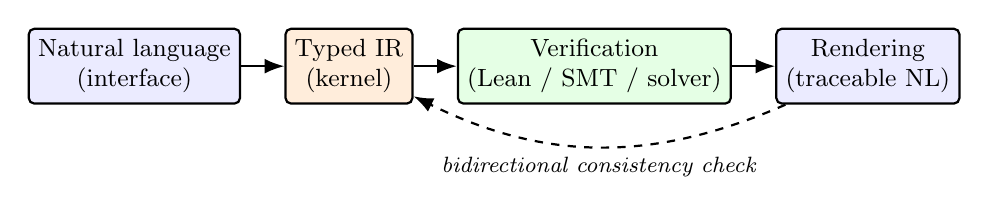
\begin{tikzpicture}[
  box/.style={rectangle,rounded corners=2pt,draw,thick,minimum height=0.95cm,align=center,font=\small},
  arr/.style={-{Latex[length=2.5mm]},thick},
  node distance=0.55cm]
  \node[box,fill=blue!8]   (nl) {Natural language\\(interface)};
  \node[box,fill=orange!14,right=of nl] (ir) {Typed IR\\(kernel)};
  \node[box,fill=green!10,right=of ir] (v) {Verification\\(Lean / SMT / solver)};
  \node[box,fill=blue!8,right=of v] (r) {Rendering\\(traceable NL)};
  \draw[arr] (nl) -- (ir);
  \draw[arr] (ir) -- (v);
  \draw[arr] (v) -- (r);
  \draw[arr,dashed,bend left=25] (r) to node[below,font=\footnotesize\itshape]{bidirectional consistency check} (ir);
\end{tikzpicture}
\end{center}

Three requirements follow from \S\ref{sec:bottleneck}: (i) the IR must be \emph{typed} (closing F2); (ii) the mapping $\rho$ must be \emph{explicit and auditable}, so that unfaithful reductions can be filtered rather than silently accepted (F1, F4); (iii) rendering back to natural language must be loss-tracked, giving traceability (F3). Draft-Sketch-Prove \citep{jiang2023draft} and DTV \citep{zhou2024dtv} are partial instantiations of this pattern---the former reduces informal proof sketches to Lean obligations, the latter to Isabelle checkable statements---and their documented failure modes are exactly the five modes of \S\ref{sec:bottleneck}, which we take as evidence for the taxonomy's completeness rather than its vacuity.

\subsection{The SRC-12 reliability checklist}\label{sec:checklist}

To make the framework actionable, we operationalize it as a 12-item checklist. Each item maps to a layer and a failure mode it guards against. The checklist is designed for a human reviewer (or an automated pipeline) auditing an AI-generated mathematical conclusion \emph{before} acting on it.

\begin{table}[h]
\centering\small
\caption{SRC-12: a reliability checklist for AI-generated mathematical conclusions.}
\label{tab:checklist}
\begin{tabular}{@{}clp{4.1cm}c@{}}
\toprule
\# & Layer & Check & Guards against \\
\midrule
1 & Gen & Is the final answer consistent across $k$ independent samples? & sampling noise \\
2 & Gen & Does the answer survive a re-derivation with a different prompt strategy? & prompt-specific shortcuts \\
3 & Gen & Is every quantity, symbol, and assumption in the problem reflected in the solution? & F1 ambiguity \\
4 & Red & Has arithmetic been delegated to a calculator/program rather than the LLM? & computation errors \citep{gao2023pal,chen2023pot} \\
5 & Red & Can each step be pointed to a formal or executable counterpart? & F3 non-invertibility \\
6 & Red & Are types and domains explicit (integers vs.\ reals, sets vs.\ tuples)? & F2 type incompleteness \\
7 & Red & Is the formalized statement checked against the original wording (paraphrase test)? & F4 vacuous formalization \\
8 & Ver & Was a symbolic tool run, and did it pass on the \emph{reduced} object? & unverified claims \\
9 & Ver & Is the checker itself versioned and reproducible (library, solver version)? & F5 format drift \citep{yang2023leandojo} \\
10 & Ver & Does the guarantee cover the claim actually made (not a weaker variant)? & overclaiming \\
11 & Both & Is there a traceable rendering of the verified object back into language? & F3 non-invertibility \\
12 & Both & Is confidence reported as a property of the \emph{process}, not the answer? & outcome-only bias \citep{uesato2022feedback} \\
\bottomrule
\end{tabular}
\end{table}

We apply SRC-12 retroactively in \S\ref{sec:limits} to bound our own claims; the checklist is also used in the accompanying AI-collaboration log to record human verification of AI-generated statements made during the preparation of this paper.

% =====================================================================
\section{Related Work}\label{sec:related}

\paragraph{Informal reasoning enhancement.} CoT prompting \citep{wei2022cot} and math-specialized pretraining \citep{lewkowycz2022minerva,azerbayev2024llemma} improve generation but change nothing at Layers 2--3; our analysis treats them as orthogonal.

\paragraph{Tool and program augmentation.} PAL and Program-of-Thoughts delegate computation to programs \citep{gao2023pal,chen2023pot}, and Toolformer learns tool invocation \citep{schick2023toolformer}. These are narrow reductions (arithmetic-level $\ir$); they verify computation but not the reasoning that constructs it.

\paragraph{Verification and search.} Verifier reranking \citep{cobbe2021gsm8k}, outcome vs.\ process supervision \citep{uesato2022feedback,lightman2024verify}, and majority voting \citep{zhou2024dtv} supply step- or answer-level signals without formal objects. Our taxonomy locates their blind spots (F1--F4).

\paragraph{Formal theorem proving.} Long before learned provers, full formalization was already used to settle major results---the Flyspeck project's formal verification of the Kepler conjecture \citep{hales2017kepler} remains a landmark. Learned provers now push this approach toward open problems: GPT-f \citep{polu2020gptf}, HyperTree Proof Search \citep{lample2022htps}, retrieval-augmented proving \citep{yang2023leandojo}, informal-guided proving \citep{jiang2023draft}, AlphaGeometry \citep{trinh2024alphageometry}, and AlphaProof \citep{hubert2025alphaproof} move reasoning into formal systems. Our contribution is not a better prover but an account of \emph{why} the informal--formal interface dominates the end-to-end reliability budget.

\paragraph{Autoformalization.} DTV \citep{zhou2024dtv} is the closest work: it demonstrates that reduction-based verification is feasible today while its filters confirm the reduction is the weak link. We generalize its lessons into a taxonomy and a checklist applicable beyond one proving environment.

% =====================================================================
\section{Discussion, Limitations, and Falsifiability}\label{sec:limits}

\paragraph{Boundary conditions.} The taxonomy in \S\ref{sec:bottleneck} is grounded in case studies from Isabelle/Lean-based systems and GSM8K/MATH-scale benchmarks; it may not transfer to settings with different unit economics, e.g., interactive proof engineering with expert users, where formal systems already dominate. The comparative analysis (\S\ref{sec:analysis}) quotes numbers from different papers trained on different base models and data; cross-paper numbers are directional evidence, not controlled comparisons. In particular, the PRM-vs-ORM gap reported by \citet{lightman2024verify} at 78.2\% vs.\ 72.4\% is explicitly \emph{not} a controlled experiment at full scale, as the authors themselves note.

\paragraph{Limitations of SRC-12.} The checklist is a judgment aid, not a guarantee; several items (e.g., item 7, the paraphrase test) require human reading, so full automation is out of reach with current tools. It has not yet been validated in a user study; measuring inter-rater agreement and time cost of SRC-12 audits is the natural next step.

\paragraph{Falsifiability.} The framework's central claim---reduction, not generation or verification, is the bottleneck---would be undermined by evidence of the following kind: (i)~systems achieving informal-language coverage \emph{and} formal guarantees \emph{without} an explicit reduction layer (e.g., end-to-end NL-to-proof models whose failures are dominated by search, not translation); or (ii)~demonstrations that learned verifiers match formal verification on trace-level error without any typed intermediate representation. Neither pattern is present in the literature we surveyed, but both are concrete and testable.

\paragraph{Ethical and societal note.} Over-trusting fluent but unverified mathematical output is already a practical hazard in education and quantitative work \citep{frieder2023chatgpt}. We release SRC-12 in the hope that even its informal use raises the cost of unverified conclusions.

% =====================================================================
\section{Conclusion}\label{sec:conclusion}

We reorganized the reliability landscape of AI mathematics around a three-layer model whose central component---semantic reduction from natural language to typed, verifiable objects---explains the observed gap between answer accuracy and reasoning validity. A taxonomy of five reduction failure modes, a cross-paper comparison of four verification architectures, and a 12-item operational checklist together turn this position into a usable framework. Reliable AI reasoning, on this account, is not \emph{generation plus a final check} but \emph{generation plus semantic reduction plus verification}---and the middle term, long implicit in every serious system, deserves to be a first-class design object.

\bibliographystyle{unsrtnat}
\bibliography{references}

\end{document}
